\documentclass[11pt]{article}
\usepackage[margin=0.8in]{geometry}
\usepackage{amsmath,amssymb,graphicx,float,hyperref}
\hypersetup{hidelinks}
\setlength{\parindent}{0pt}
\setlength{\parskip}{5pt}
\begin{document}
\begin{center}
{\Large ECE276C Assignment 1}\\[3pt]
{\large Robot Kinematics and Simple Control}
\\[8pt]
Sachin Bhadang\\
PID: A69040722\\
Email: \href{mailto:sbhadang@ucsd.edu}{sbhadang@ucsd.edu}
\end{center}

\section*{1. Arm and body-fixed coordinate frames}
\begin{figure}[H]
\centering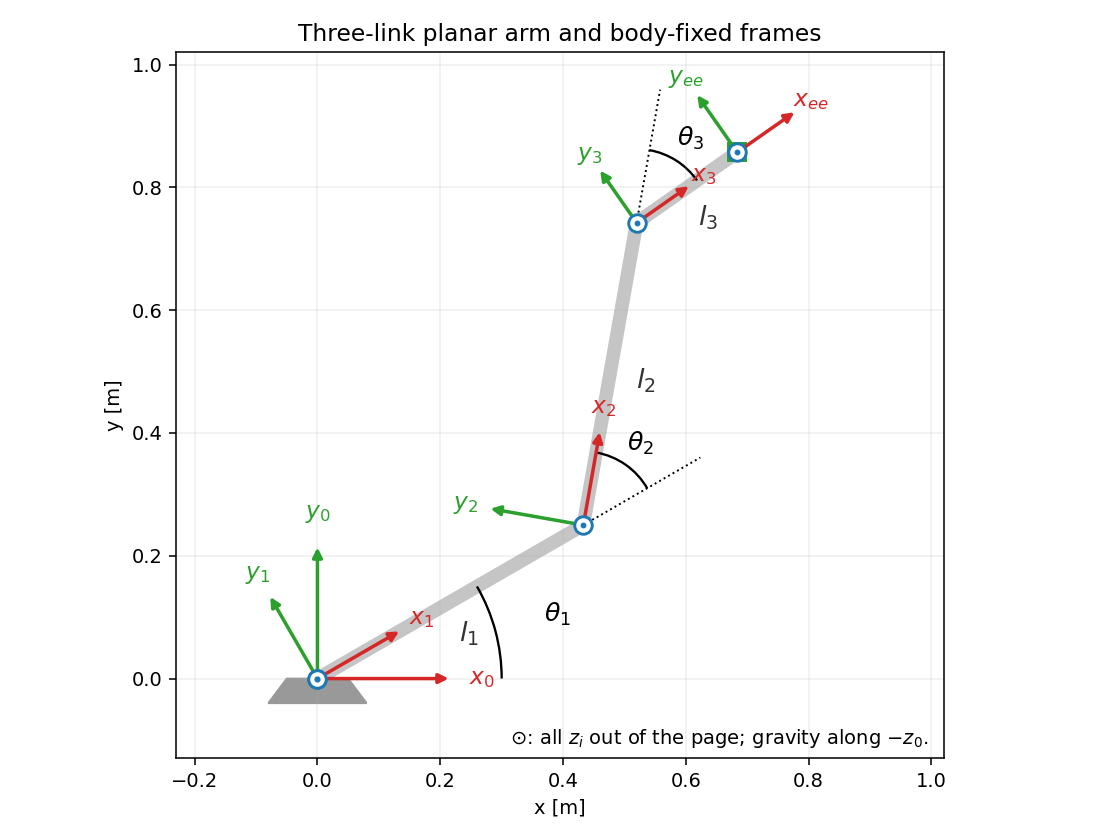
\includegraphics[width=0.65\textwidth]{results/q1_frames.png}
\end{figure}
Frame $\{0\}$ is fixed at the base. Frame $\{i\}$ is attached to link $i$ at joint $i$, with $x_i$ along the link and $z_i$ along the joint axis. Frame $\{ee\}$ is at the tip, with the same orientation as $\{3\}$. All frames are right-handed. The offsets follow assignment Table 1: $a_0=0$, $a_1=l_1$, $a_2=l_2$, $a_3=l_3$.

\section*{2. End-effector kinematics}
Let $\mathbf{q}=[\theta_1,\theta_2,\theta_3]^\top$ and $\mathbf{x}=f(\mathbf{q})=[X,Y,\theta]^\top$. Then
\begin{align*}
X &= l_1\cos\theta_1+l_2\cos(\theta_1+\theta_2)
     +l_3\cos(\theta_1+\theta_2+\theta_3),\\
Y &= l_1\sin\theta_1+l_2\sin(\theta_1+\theta_2)
     +l_3\sin(\theta_1+\theta_2+\theta_3),\\
\theta &= \theta_1+\theta_2+\theta_3 \pmod{2\pi}.
\end{align*}
At $\mathbf{q}=\mathbf{0}$, the arm points along $+x_0$ and the tip is at $(l_1+l_2+l_3,0)$.

\newpage
\section*{3. Required PyBullet configurations}
\begin{figure}[H]
\centering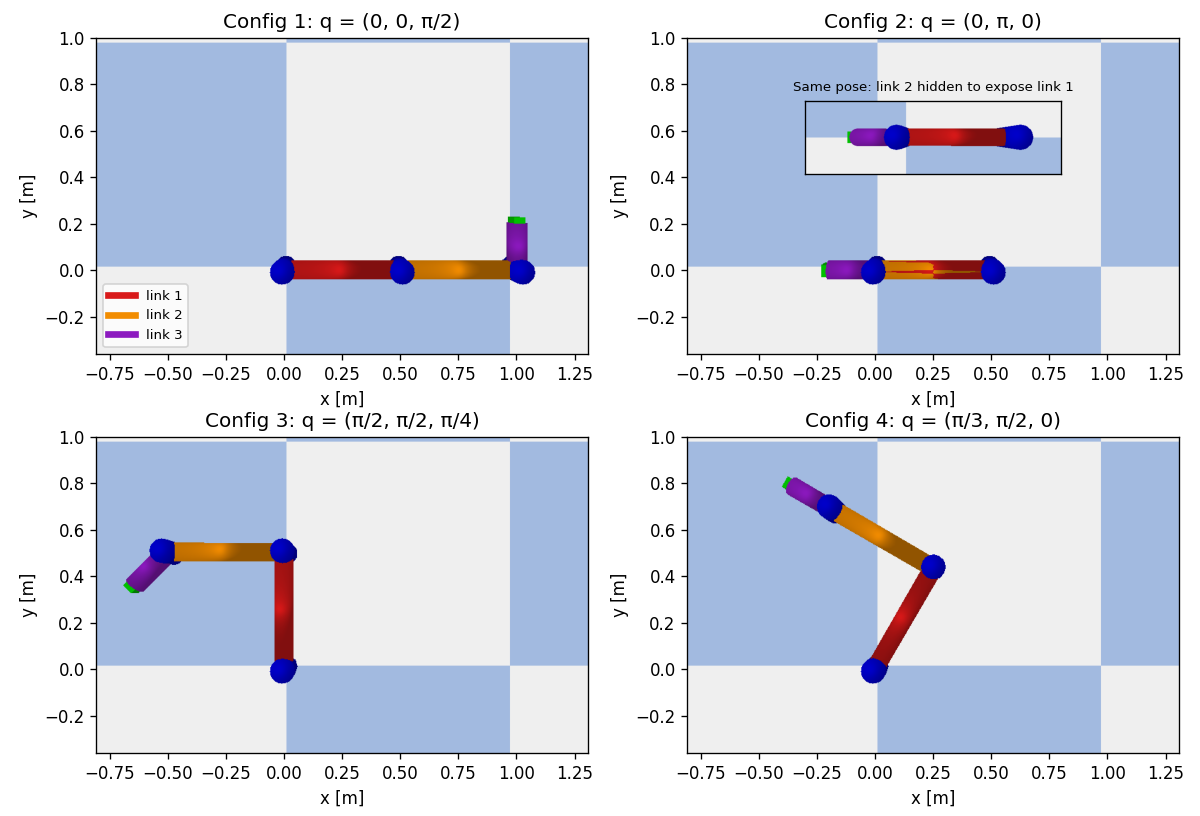
\includegraphics[width=0.85\textwidth]{results/q3_configs.png}
\caption{The supplied URDF with $l_1=l_2=0.5$\,m and $l_3=0.2$\,m. Links 1, 2 and 3 are red, orange and purple. In configuration 2, links 1 and 2 coincide exactly; the labeled inset hides link 2 to expose link 1 without changing the joint configuration.}
\end{figure}

\section*{4. Open-loop and closed-loop control diagrams}
\begin{figure}[H]
\centering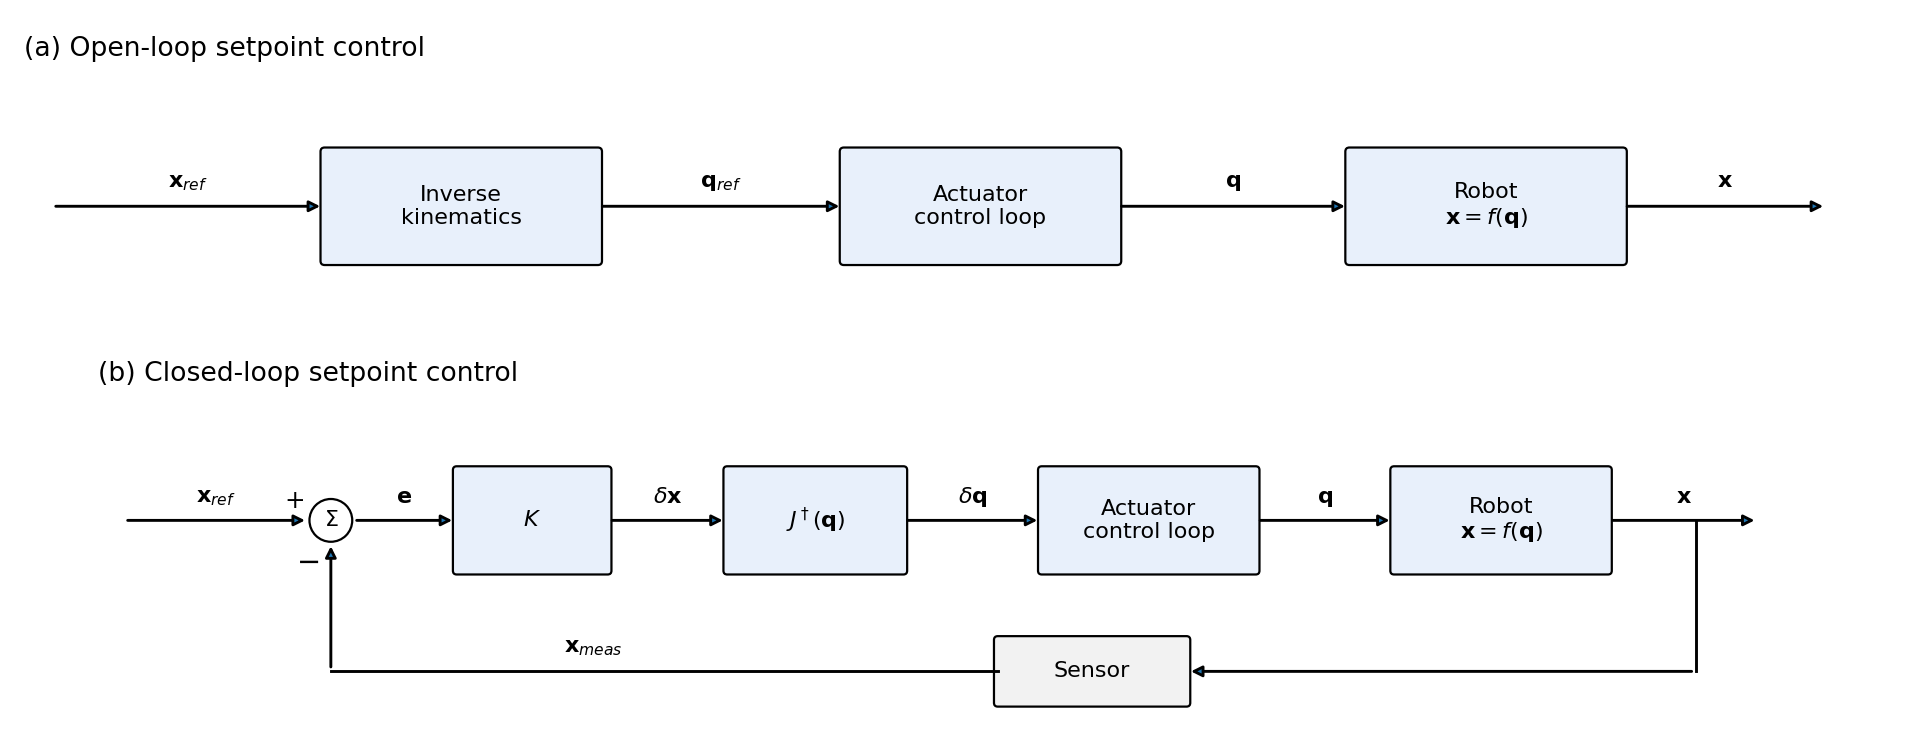
\includegraphics[width=\textwidth]{results/q4_block_diagrams.png}
\end{figure}
Both diagrams use $\mathbf{x}_{ref}=[X,Y,\theta]_{ref}^\top$.
In (b), $J=\partial f/\partial\mathbf{q}\in\mathbb{R}^{3\times3}$,
$\mathbf{e}=\mathbf{x}_{ref}-\mathbf{x}_{meas}$, and the orientation error is wrapped to $[-\pi,\pi)$.

\newpage
\section*{5. Smooth profile and open-loop motion}
For a move of duration $T$, let $\tau=t/T$ and use
\[
\mathbf{x}_{ref}(t)=\mathbf{x}_0+s(\tau)(\mathbf{x}_f-\mathbf{x}_0),
\qquad s(\tau)=10\tau^3-15\tau^4+6\tau^5.
\]
The polynomial satisfies the boundary conditions
\[
s(0)=0,\quad s(1)=1,\quad
s'(0)=s'(1)=0,\quad s''(0)=s''(1)=0,
\]
where primes denote derivatives with respect to $\tau$. In physical time,
\[
\dot s=\frac{30\tau^2(1-\tau)^2}{T},\qquad
\ddot s=\frac{60\tau(1-\tau)(1-2\tau)}{T^2}.
\]
The profile is second-order smooth ($C^2$): position, velocity and acceleration are continuous, including at the waypoints. All coordinates use the same $s$, so each Cartesian segment is straight.

The four moves $1\to2\to3\to4\to1$ take $2.5$\,s each, totaling $10$\,s; $\theta_{ref}=0$ throughout. At $240$\,Hz, analytic inverse kinematics converts each sampled pose into joint setpoints on one continuous elbow branch. These drive PyBullet's position motors, with joint velocity feedforward; measured end-effector pose is used only for recording.

\begin{figure}[H]
\centering
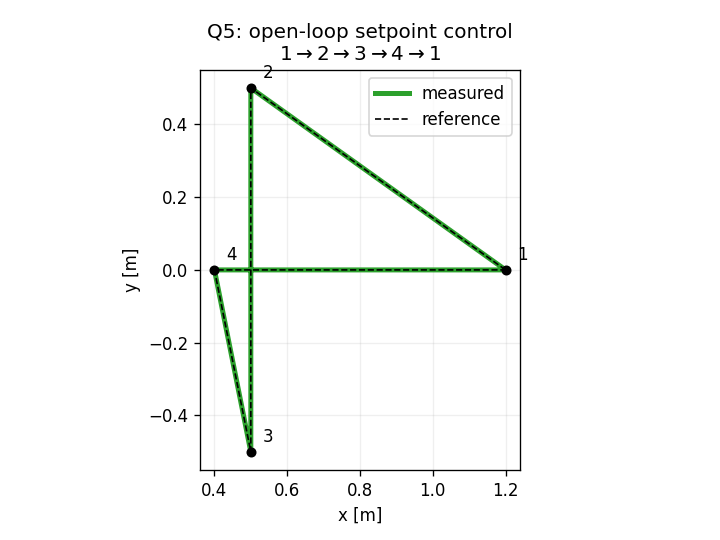
\includegraphics[width=0.36\textwidth]{results/q5_open_loop.png}\\[4pt]
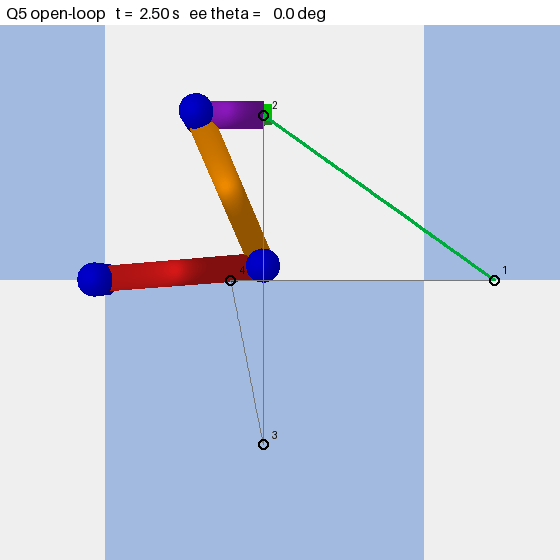
\includegraphics[width=0.32\textwidth]{results/q5_open_loop_frame1.png}\hfill
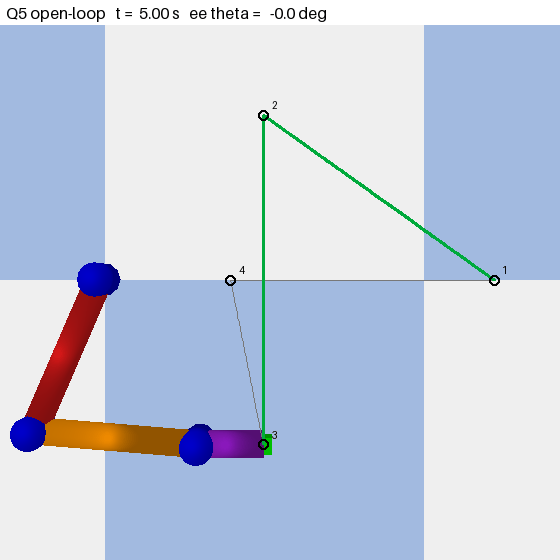
\includegraphics[width=0.32\textwidth]{results/q5_open_loop_frame2.png}\hfill
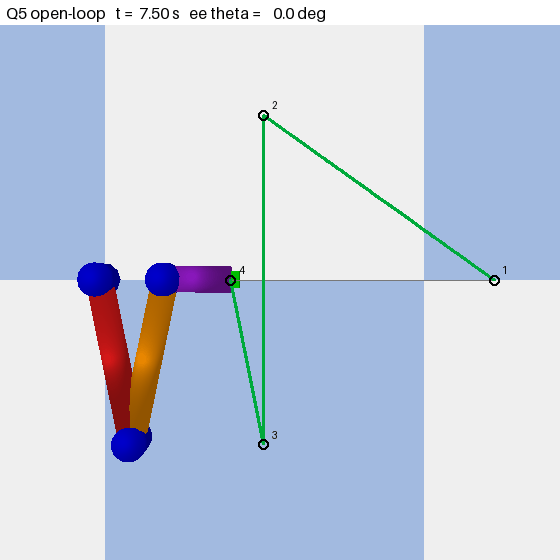
\includegraphics[width=0.32\textwidth]{results/q5_open_loop_frame3.png}
\caption{Q5: measured end-effector path (top) and animation frames at $t=2.5$, $5.0$ and $7.5$\,s (bottom, left to right), reaching locations 2, 3 and 4 with $\theta=0$.}
\end{figure}
Animation: \texttt{q5\_open\_loop.gif} ($20$\,fps, $10.05$\,s including the final frame). The reference velocity is zero at every waypoint. In the sampled simulation, waypoint speeds are below $6\times10^{-5}$\,m/s and the maximum position error is $3.9\,\mu$m.

\newpage
\section*{6. Closed-loop motion and nullspace control}
The task is now $\mathbf{x}_{xy}=[X,Y]^\top$; $\theta$ is free. Use the same reference path and timing as Q5, with
$J_{xy}=\partial\mathbf{x}_{xy}/\partial\mathbf{q}\in\mathbb{R}^{2\times3}$.
Compute the SVD pseudoinverse $J_{xy}^\dagger$ and
\[
N=I_3-J_{xy}^\dagger J_{xy},\qquad J_{xy}N=0.
\]

Define the interior angles at the shared joints by
\[
\alpha_{12}=\pi-|\bar\theta_2|,\qquad
\alpha_{23}=\pi-|\bar\theta_3|,
\qquad \bar\theta_i=\operatorname{wrap}_{[-\pi,\pi)}(\theta_i).
\]
A straight pair of links has the largest interior angle, $\pi$. To drive both angles toward this value subject to the position constraint, minimize their squared departures from $\pi$:
\[
U(\mathbf{q})=\tfrac12\big[(\pi-\alpha_{12})^2+(\pi-\alpha_{23})^2\big]
=\tfrac12(\bar\theta_2^2+\bar\theta_3^2),\qquad
\nabla_{\mathbf{q}}U=[0,\bar\theta_2,\bar\theta_3]^\top.
\]
The angles stay away from the wrap discontinuity during this motion. Use projected gradient descent:
\[
\dot{\mathbf{q}}_2=-\lambda\nabla_{\mathbf{q}}U,\qquad
\dot{\mathbf{q}}_{null}=N\dot{\mathbf{q}}_2,\qquad \lambda=10\,\mathrm{s}^{-1}.
\]
Combining it with the next-sample closed-loop trajectory step gives
\[
\delta\mathbf{q}
=J_{xy}^\dagger\big(\mathbf{x}_{xy,ref}[k+1]-\mathbf{x}_{xy,meas}[k]\big)
+\Delta t\,\dot{\mathbf{q}}_{null},\qquad \Delta t=1/240\,\mathrm{s}.
\]
Thus $J_{xy}\dot{\mathbf{q}}_{null}=0$: the secondary controller changes posture without adding Cartesian velocity. This is a local optimization of $U$ along the position constraint.

The implementation reads the joint angles and end-effector position each step. It corrects the finite-step linearization error with repeated Jacobian position corrections, then sends the resulting joint increment divided by $\Delta t$ to the velocity motors. At location 1 the arm is straight and $J_{xy}$ is singular; analytic IK selects the first nonzero departure sample, and the final sample returns to the straight posture. The simulated initial state is exactly $\mathbf{q}=\mathbf{0}$.

\begin{figure}[H]
\centering
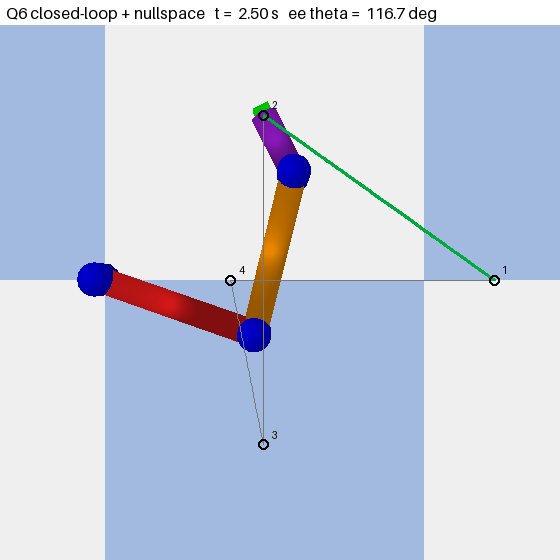
\includegraphics[width=0.32\textwidth]{results/q6_closed_loop_frame1.png}\hfill
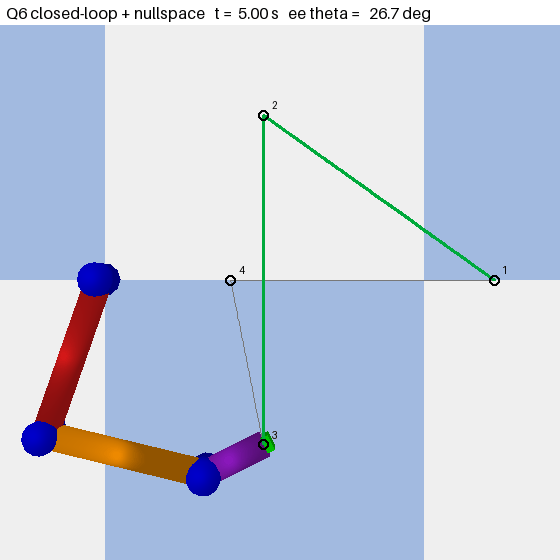
\includegraphics[width=0.32\textwidth]{results/q6_closed_loop_frame2.png}\hfill
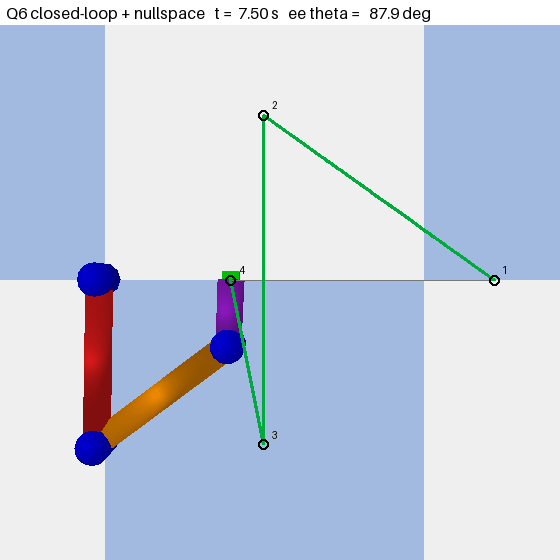
\includegraphics[width=0.32\textwidth]{results/q6_closed_loop_frame3.png}
\caption{Q6 animation frames at $t=2.5$, $5.0$ and $7.5$\,s (left to right). The same locations are reached while orientation is free.}
\end{figure}
Animation: \texttt{q6\_closed\_loop.gif} ($20$\,fps, $10.05$\,s). The maximum measured position error is below $2\,\mu$m. The nullspace identity is exact in the kinematic model; the simulation follows the prescribed path to this numerical accuracy.
\end{document}
